\chapter{Wearing the Crown of Mathematics}
We can simply, but reasonably correctly, claim that there are three fundamental building blocks of mathematics: numbers, geometric figures and logical reasoning. Just as geometric objects and mathematical statements can be thought of as systematic collections of points and words, so can integers be broken into their indivisible components known as prime numbers. We have already discussed the logical reasoning part in form of algebra and combinitorics, let's talk about numbers now.\\
Welcome to Number Theory considered by many as the “crown of mathematics”\\
\begin{example}
    Prove that $1^n+2^n+3^n+\dots+(n-1)^n$ is divisible by $n$ for all odd $n$.
\end{example}
A human calculator(or a machine one for that matter) can compute to maybe $n=50$, but that is not even $1\%$ of $\infty$ for which the proposition must hold.\\
In contrast, using number theory we can proves this claim to be true within seconds, using only two lines and almost no calculations. How? You'll understand by the end of the chapter. While this question is quite easy, I reckon that some of you know how to solve it, number theory is not always that easy.\\
\begin{example}
    (IMO 1988, P6) Let $a$ and $b$ be positive integers such that $ab + 1$ divides $a^{2} + b^{2}$. Show that $\frac {a^{2} + b^{2}}{ab + 1}$ is the square of an integer.
\end{example}
Even though this may look overall like some sort of a “simple division exercise,”, it is a lot worse. This is believed to be the hardest IMO question of all time. The problem was solved perfectly by only 12 students at the IMO, and very few partial scores were given: it was “all or nothing.” But this is not even a taste of the complexity and beauty of number theory. Any work about number theory would be incomplete if we don't mention perhaps the greatest math question.\\
\begin{theorem}
    [Fermat's Last Theorem]
    $a^n+b^n \neq c^n$ for $n>2$
\end{theorem}    
This theorem may seem innocent enough. But its proof was a mystery for more than $350$ years. The theorem was written in the margin of a book by Piree de Fermat in 1637. He claimed to have “a truly marvelous proof of this proposition which this margin is too narrow to contain". He never wrote the proof down, and the answer to this was lost to time.\\
It was proven by Andrew Wiles in 1995. Anyone who even remotely knows about Wiles’s actual proof will tell you that it is impossible to describe it in a few easy-to-understand sentences(it is 100+ pages long and mathematically dense). In fact, it is well beyond the scope of this book or of any highschool or undergraduate facing textbook and becomes accessible only in an advanced graduate course on modular forms. Do I wish to write a book on it one day? YES. Will that day be today? NO.\\
The amazing thing is that most of this advance math wasn't available to Fermat in 1637, and we have reason to believe that he really had a proof. Fermat scribbled a lot of mathematical claims in the margins, and all of them were eventually proven using 17th century math. This was the only exception. It was Fermat's last theorem to be left unproven. While Wiles's proof is an achievement in its own regard, we still don't know how Fermat would have proven this.\\
Fermat's mathematical knowledge was similar to that of Olympiad mathematics. Which raises the question: Could you be the high school mathematician to find the elementary proof which has evaded the community for centuries? Who knows? But before we are even capable of approaching such a problem, let's actually learn the tools we would need.\\
\section{Division}
I expect you to be familiar with division in the form:\\
\begin{figure} [h]
    \centering
    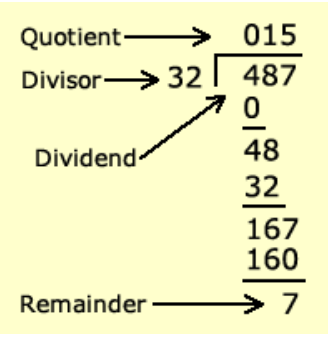
\includegraphics[width=0.5\linewidth]{Photos/Long Divison.png}
    \caption{The long division}
\end{figure}
You must also know that:\\
\begin{theorem}
    $a = qd+r$ such that $0 \leq r <|d|$\\
    Where $q,r$ are uniquely determined for $a,b$
\end{theorem}
 Do we notice any concepts whose appearance seems striking or “unjustified”? The absolute value $|d|$ jumps out at us: why do we need it? Well, if we divide by a negative $d$, we still want to arrive at a non-negative remainder $r$, but the inequalities $0 \leq r<d< 0$ won’t make much sense! This is remedied by the absolute value $|d| > 0$. For example, dividing $13$ by $-5$ yields $13 = (-2) \cdot (-5) + 3$: the remainder $3$ satisfies $0 \leq 3 < |-5|$\\
 \begin{definition}
     If $a = qd$ for some non-zero integers $a, d,$ and $q$, we say that $d$ and $q$ divide $a$, or that $d$ and $q$ are divisors or factors of $a$, and write $d | a$ and $q | a$. Further, we say that $d | 0$ since $0 = d · 0$
 \end{definition}
For instance, $5 | 10$, but $5 \nmid 13$. Note that the bar in "d | a" is vertical, not slanted; while $5/10$ stands for the usual fraction $\frac{1}{2}$, the expression "5 divides 10" means something different, so be careful! Also, another trivial observation: if $d | a$, it is not necessarily true that $d \leq a$; indeed, $7 | (-14)$ but $7 > -14$. To avoid annoying minus signs, we conclude in general that $d | a$ implies $|d| \leq |a|$ (unless $a = 0$).\\
We also need to note that division is just repeated addition or subtraction(whatever approaches 0). For example for $a=16, d=6$, we can find the remainder by $16 \to 16-6 \to 10-6 \to 4$. However, for $a=-19, d=5$, we find the remainder by $-19 \to -19+5 \to -14+5 \to -9+5 \to -4+5 \to 1$.\\
We stopped the moment the condition $0 \leq r <|d|$ became true. This is called the Euclidean Algorithm for division.\\
We'll use this algorithm to prove our theorem.\\
\begin{proof}
Proof of existence: Set $r$ to be the smallest non-negative such difference, say, $r = a - qd$ for some $q$. Since we start with a positive $a$ and decrease it by $d$ each time, we will eventually plunge under $0$: the difference right before this plunge is our $r$. Rewriting, we have $a = qd + r$ with $r \geq 0$. Thus, we have constructed our quotient $q$ and remainder $r \geq 0$; we only need to verify that $r < d$.\\
To the contrary, suppose $r \geq d$. Say we had $12$ apples to give to $5$ people. After giving everyone one apple, we are left with $7$. If we kept them as remainder, we are greedy. We give the people one more each and have $2$ as remainder. In general, we can subtract another $d$ from $r$ and get an even smaller non-negative difference: 
\[a - qd = r \rightarrow a - (q + 1)d = r - d \geq 0,\]
which contradicts our choice for $a - qd$ as the smallest such difference. We conclude $r < d$. Hence we have constructed the desired quotient $q$ and remainder $r$. We can symmetrically prove this for $a$ or $d$ being negative.\\
Proof of uniqueness: Let's to the contrary assume that $q$ and $r$ are not unique for every $a$ and $d$.\\
We suppose that in addition to one quotient $q$ and remainder $r$, there is another non equal quotient $q_1$ and remainder $_r1$:
$a = qd + r = q_1d + r_1\\
\iff r-r_1=d(q-q_1)\\
\iff d|(r-r_1)\\
\iff |r-r_1| \geq d$\\
Which is untrue for all $r \neq r_1$ by the fact that $0 \leq r < |d|$\\
Hence, by contradiction, $r=r_1$ and $q=q_1$.\\
\end{proof}
Note that this is often how we prove existence and uniqueness of something.\\
While this may seem excessive proving an obvious theorem, this is foundation for a lot more complex proves and without certainty of its truth, everything built on its foundation is shaky at best.\\
We will also take this moment to define two new functions:\\
\begin{definition}
[Greatest Common Divisor(GCD)]
If we take $F_a$ to be the set of all factors of $a$ and $F_b$ to be the set of all factors of $b$
    $\gcd(a,b)= \max( F_a \cap F_b)$
\end{definition}
\begin{definition}
[Least Common Multiple(LCM)]
If we take $M_a$ to be the set of all multiples of $a$ and $M_b$ to be the set of all multiples of $b$
    $\lcm(a,b)= \min( F_a \cap F_b)$
\end{definition}
We can basically find the GCD using the Euclidean algorithm as follows:\\
For two natural $a, b$ such that $a > b$, to find
\begin{theorem}
$\gcd(a, b)$ we use the division algorithm repeatedly:\\
$a = bq_1 + r_1\\
b = r_1q_2 + r_2\\
r_1 = r_2q_3 + r_3\\
\vdots\\
r_{n-2} = r_{n-1}q_n + r_n\\
r_{n-1} = r_nq_{n+1}.$\\
Then we have $\gcd(a, b) = \gcd(b, r_1) = \gcd(r_1, r_2) = \dots = \gcd(r_{n-1}, r_n) = r_n$\\
\end{theorem}
This can be proven simply by using the definition of GCD and the Euclidean algorithm.\\
Another thing to notice is that $\lcm(a,b)\cdot \gcd(a,b)=ab$. It's proof follows from $a=kx$ and $b=ky$ where $x,y$ are coprime(or have $\gcd(x,y)=1$)\\
We can also use these functions to prove a theorem which we'll use a lot later.\\
\begin{theorem}
    [Bezout's Theorem] 
    For $a, b \in \mathbb{N}$, there exist $x, y \in \mathbb{Z}$ such that $ax + by = \gcd(a, b)$
\end{theorem}
\begin{proof}
    The proof is simply by running the Euclidean Algorithm backwards.
    $\gcd(a, b) = r_{n-2} - r_{n-1}q_n\\
    = r_{n-2} - (r_{n-3} - r_{n-2}q_{n-1})q_n\\
    = r_{n-2}(1 + q_nq_{n-1}) - r_{n-3} (q_n)\\
    = \vdots\\
    = ax + by.$\\
\end{proof}
This result must not be that fun. But a rather surprising, and beautiful, result is:\\
\begin{theorem}
    $\gcd(a^m-1, a^n-1)=a^{\gcd(m,n)}-1$
\end{theorem}
\begin{proof}
    We can prove this by simply using the algebraic fact that $a^k-1|a^m-1$ if $k|m$, which follows from the sum of GP formula or the general difference expansion(whichever you like).\\
    The GCD will happen for the largest $k$ such that $k | m,n \iff k=\gcd(m,n)$\\
    Hence, $\gcd(a^m-1, a^n-1)=a^{\gcd(m,n)}-1$.\\
\end{proof}
\section{Congruence Modulo}
Before today when we divided two numbers, our interest used to lie in the quotient. But sometimes, remainders become much, much more useful. Once something becomes useful, we give it some respect. Hence, instead of using remainder as if it is leftover soup, we start calling it congruence modulo or modulo. 
\begin{definition}
    $r \equiv a \pmod d)$ means that $a$ leaves remainder $m$ when divided by $d$.
\end{definition}
This definition of modulo leads us to some of its fundamental properties. These are all trivial to see and I expect that you will be able to prove them quite easily.
\begin{theorem}
\begin{enumerate}
    \item \textbf{Reflexivity:} $a \equiv a \pmod{n}$\\
    \item \textbf{Symmetry:} $a \equiv b \pmod{n}$ if and only if $b \equiv a \pmod{n}$ \\
    \item \textbf{Transitivity:} If $a \equiv b \pmod{n}$ and $b \equiv c \pmod{n}$, then $a \equiv c \pmod{n}$\\
\end{enumerate}    
\end{theorem}
These three define the nature of the modulo function, which allows us to state:
\begin{theorem}
\begin{enumerate}
    \item \textbf{Compatibility with Translation:} $a + k \equiv b + k \pmod{n}$ for any integer $k$\\
    \item \textbf{Compatibility with Scaling:} $ka \equiv kb \pmod{n}$ for any integer $k$\\
    \item We can also state it as: $ka \equiv kb \pmod{kn}$ for any integer $k$\\
    \item \textbf{Compatibility with Exponentiation:} $a^k \equiv b^k \pmod{n}$ for any non-negative integer $k$
    \item \textbf{Compatibility with Addition:} $a_1 + a_2 \equiv b_1 + b_2 \pmod{n}$
    \item \textbf{Compatibility with Subtraction:} $a_1 - a_2 \equiv b_1 - b_2 \pmod{n}$
    \item \textbf{Compatibility with Multiplication:} $a_1 \cdot a_2 \equiv b_1 \cdot b_2 \pmod{n}$
    \item \textbf{Compatibility with Polynomial Evaluation:} $p(a) \equiv p(b) \pmod{n}$, for any polynomial $p(x)$ with integer coefficients

\end{enumerate}
\end{theorem}
Compatibility with exponentiation is used in questions a lot. Here are two examples:\\
\begin{example}
    (a)Find the remainders of $2^{1998}$ divided by $3$ and $3^{1998}$ when divided by $2$.\\ 
    (b)Find the remainders of $5^{2007}$ divided by $7$ and of $17^{1701}$ divided by 11.\\
\end{example}
\begin{proof}
    [Solution]
    For (a), we can easily notice that $2 \equiv -1 \pmod{3}$, therefore $2^{1998} \equiv -1^{1998} \pmod{3} = 1 \pmod{3}$\\
    The second one is even worse as $3 = 1 \pmod{2}$, which makes $3^{1998} \equiv 1^{1998} \pmod{2} = 1 \pmod{2}$\\
    For (b), we need to notice that $5^3 = 125 \equiv -1 \pmod{7}$ which solves the question as $\frac{2007}{3}=669$. This makes $5^{2007}=125^{669}\equiv -1^{669} \pmod{7}\equiv -1 \pmod{7}\equiv6 \pmod{7}$\\
    The second one is more like it. Consider $\pmod{11}$ to be applicable throughout the solve and $=$ and $\equiv$ be interchangeable:\\
    $17^{1701}=6^{1701}\\
    =6*36^{850}=6*3^{850}=6*9^{425}\\
    =54*9^{424}=-1*81^{212}=-1*7^{212}=-1*49^{106}\\
    = -1*5^{106}= -1*25^{53}=-1*3^{53}\\
    =-3*3^{52}= -3*9^{26}=-3*81^{13}\\
    =-3*4^{13}=-12*4^{12}=-1*16^{6}\\
    =-1*5^{6}=-1*25^{3}=-1*3^3=26=4$\\
    Hence the remainder is 4.\\
\end{proof}
The part 2 of (b) is the common type of modulo you can expect to occur often. The other were designed for elegant solutions. \\
We can also use the compatibility of exponentiation to get the following result: the units digit, tens digit or any place per say, of any power repeats in cycles, this can be proven by taking $d$ as $10$, then $100$ and so on.\\
Here is an example for you to try.
\begin{example}
(AIME 2010)
    Find the remainder when $9 \times 99 \times 999 \times \cdots \times \underbrace{99\cdots9}_{\text{999 9's}}$ is divided by $1000$.
\end{example}
As we close this section, with our new found knowledge, we are now capable enough to prove the first example.\\
\begin{proof}
    $1^n+2^n+\dots+(n-1)^n$\\
    We take $\pmod{n}$ to get $1^n+2^n+\dots+(-2)^n+(-1)^n$\\
    as $n$ is odd, $1^n-1^n+2^n-2^n+\dots \equiv 0 \pmod{n}$, which means that $1^n+2^n+\dots+(n-1)^n$ is divisible by $n$.\\
\end{proof}
We just proved something about numbers, with powers and sums, without computing a single one. That's quite impressive, isn't it?\\
We'll return to Congruence modulo in the next chapter.\\
\section{Prime Numbers}
\begin{example}
    There are 100 light bulbs on the wall, all of them initially lit up. Following specific rules:
    \begin{enumerate}
        \item The first bulb overheats and breaks.
        \item A math God decides that bulbs with even numbers (except for 2) will burst.
        \item A physics God decides that bulbs divisible by 3 (except for 3) will explode.
        \item A chemistry God decides that bulbs divisible by 5 (except for 5) will turn into glass shards.
        \item A biology God decides that bulbs divisible by 7 (except for 7) will shatter.
    \end{enumerate}
After all these divine interventions, how many lights remain illuminated? (Note: Once a bulb is affected, it cannot be restored by any other divine power.)
\end{example}
You'll be sad to know that we don't have any way to solve this without actually writing the numbers down. As it turns out, after crossing the broken bulbs out, we get:\\
\begin{figure}[h]
    \centering
    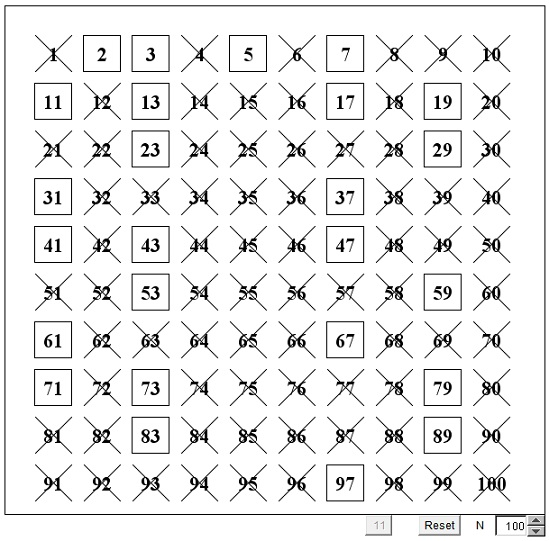
\includegraphics[width=0.5\linewidth]{Photos/Prime Sieve.png}
    \caption{The bulbs which remain lit. The diagram is called the Sieve of Eratosthenes}
\end{figure}
What we'll notice is that all the bulbs which remain have exactly two divisors or factors: $1$ and the
number itself. These numbers are called the prime numbers. The crossed out numbers are called the composite numbers\\
\begin{theorem}
    [Fundamental Theorem of Arithmetic]
    Every natural number $n \neq 1$ may be prime factorized in one and only one way as $p_1^{e_1}p_2^{e_2}\dots p_k^{e_k}$ where all $p$ are prime and all $e \in \mathbb{N}$.
\end{theorem}
This is another theorem which is quite simple and known to every schoolchild. The only problem, schools don't teach the proof, which is essential for deeper understanding. I have discussed the proof below.\\
\begin{proof}
    We divide it into two parts. Showing the existence of a prime factorization and then proving it's uniqueness.\\
    Proof of existence: (B) Prime factorization trivially exists for the first few numbers. Let's consider till $n=4$ where $2,3$ are prime and $4=2^2$.\\
    (S) Let's assume that all numbers less than $k$ can be prime factorized. If $k$ is prime, the number has a trivial prime factorization, $k=k^1$. If $k$ is composite, which means $k=pq$ where $p$ and $q$ are less than $k$ and have a prime factorization. We multiply the prime factorization to get the prime factorization of $k$.\\
    Proof of uniqueness: Let's to the contrary assume that:\\
    $p_1^{e_1}p_2^{e_2}\dots p_k^{e_k}=q_1^{f_1}q_2^{f_2}\dots q_l^{f_l}$ where terms of both $p,q$ are distinct primes.\\
    We can say that as $p_1$ divides the LHS, it also divides the RHS. This means some $q$ is divisible by $p_1$, let that term be $q_1$. However, as $p_1$ and $q_1$ are primes, $p_1=q_1$. This leads to $p_i=q_i$ for $i \leq k=l$. This also leads to the exponents being equal, which makes the prime factorization exactly the same, contradicting the initial assumption.\\
    Thus, the assumption was false. This means that every $n$ has one and only one prime factorization of the form $p_1^{e_1}p_2^{e_2}\dots p_k^{e_k}$\\
\end{proof}
This leads to the observation that in order to check whether a number $n$ is prime, we need to check all the primes that are less than or equal to $\sqrt{n}$ as any factor of $n$ less than $\sqrt{n}$ has its corresponding factor greater than $\sqrt{n}$ and the same is true vice versa.\\
\begin{example}
    How many prime numbers are there? Prove it!
\end{example}
Note that we have 25 primes less than 100. But only 21 from 100 to 200. It drops to 16 in the range 200 to 300. So a question arises, are their finite primes?\\
NO, and we'll prove that.
\begin{proof}
    Let's, to the contrary, assume that we have finite primes. We can list them as $p_1, p_2, \dots$. However, $(p_1*p_2*\dots)+1$ is not divisible by any of them. If it is a prime, our list is incomplete. If it is not, its prime factors have been left out from the list. In either case, we have a contradiction. Hence, our initial assumption was false. Thus, we have infinite primes.
\end{proof}
This is one of the most beautiful proofs in math, considered to be the part of \textbf{"THE BOOK"}.\\
We normally denote primes with $p$. While we can prove that there are infinite primes, it is an open question if there are infinite primes of the form $p+2$ called Euclidian Primes, infinite primes of the form $2p+1$ called Germain Primes or infinite primes of the form $2^p-1$  called Mersenne Primes. While proving these is much harder, I do recommend thinking about it when you get time.\\
Another common question is if we have some formula to find the $n^{th}$ prime. Unfortunately, no such formula exists which is accurate, the best one is called Prime Number Theorem. It uses the famous Riemann Zeta function and a lot of math beyond this book to get the following result:
\begin{theorem}
[Prime Number Theorem]
    Number of primes less than $n \approx \frac{n}{\ln{n}}$\\
    and consequently, the $n^{th}$ prime $ \approx n \ln{n}$
\end{theorem}
They both are inaccurate for small $n$ and become increasingly accurate as $n \to \infty$\\
NOTE: The prime number theorem is included just for your information, it will never be used in any competition, in any way whatsoever. So you can totally read and forget it.\\
\section{Number Bases}
To understand the notion of number bases, we look at our own number system. We use the decimal(dec), or base $10$, number system. To help explain what this means, consider the number $2746$. This number can be rewritten as $2746_{10}=2\cdot10^3+7\cdot10^2+4\cdot10^1+6\cdot10^0.$\\
Note that each number in 2746 is actually just a placeholder which shows how many of a certain power of 10 there are. The first digit to the left of the decimal place (recall that the decimal place is to the right of the $6$, i.e. $2746.0$) tells us that there are six $10^0$'s, the second digit tells us there are four $10^1$'s, the third digit tells us there are seven $10^2$'s, and the fourth digit tells us there are two $10^3$'s.\\
Base-10 uses digits 0-9. Usually, the base, or radix, of a number is denoted as a subscript written at the right end of the number. We don't really do that with base $10$ as it is the one we use all day. If we did, we would write the above example as $2746_{10}$, where $10$ is the radix.\\
The next natural question is: how do we convert a number from another base into base $10$? For example, what does $4201_5$ mean? Just like base $10$, the first digit to the left of the decimal place tells us how many $5^0$'s we have, the second tells us how many $5^1$'s we have, and so forth. Therefore:\\
$4201_5 = (4\cdot 5^3 + 2\cdot 5^2 + 0\cdot 5^1 + 1\cdot 5^0)_{10}$\\
$=4\cdot 125 + 2\cdot 25 + 1$
$= 551_{10}$\\
From here, we can generalize. Let $x=(a_na_{n-1}\cdots a_1a_0)_b$ be an $n+1$-digit number in base $b$. In our example ($2746_{10}$) $a_3 = 2, a_2 = 7, a_1 = 4$ and $a_0 = 6$. We convert this to base 10 as follows:\\
$x = (a_na_{n-1}\cdots a_1a_0)_b$\\
$= (b^n\cdot a_n + b^{n-1}\cdot a_{n-1}+\cdots + b\cdot a_1 + a_0)_{10}$\\
However, it turns out that converting from base 10 to other bases is far harder for us than converting from other bases to base 10. This shouldn't be a surprise, though. We work in base 10 all the time so we are naturally less comfortable with other bases. Nonetheless, it is important to understand how to convert from base 10 into other bases.\\
\begin{example}
    Convert $1000_{10}=n_7$, Find the value of $n$. 
\end{example}
Basically we are looking for a solution to \\
$1000 = a_0 + 7a_1 + 49a_2 + 343a_3+2401a_4+\cdots$\\
where all the $a_i$ are digits from 0 to 6. Obviously, all the $a_i$ from $a_4$ and up are 0 since otherwise they will add in a number greater than 1000, and all the terms in the sum are non negative. Then, we wish to find the largest $a_3$ such that $343a_3$ does not exceed 1000. Thus, $a_3= 2$ since $2a_3=686$ and $3a_3=1029$. This leaves us with\\
$1000 = a_0 + 7a_1 + 49 a_2 + 343(2)\\
\iff 314 = a_0 + 7a_1 + 49 a_2.$\\
Using similar reasoning, we find that $a_2 = 6$, leaving us with\\
$20 = a_0 + 7a_1.$\\
We use the same procedure twice more to get that $a_1=2$ and $a_0=6$.\\
Finally, we have that $1000_{10}=2626_7$.\\
An alternative version is to find the "digits" $a_0,a_1,\dots$ starting with $a_0$. Note that $a_0$ is just the remainder of division of $1000$ by $7$. So, to find it, all we need to do is to carry out one division with remainder. We have $1000:7=142(R6)$. How do we find $a_1$, now? It turns out that all we need to do is to find the remainder of the division of the quotient $142$ by $7$: $142:7=20(R2)$, so $a_1=2$. Now, $20:7=2(R6)$, so $a_3=6$. Finally, $2:7=0(R2)$, so $a_4=2$. We may continue to divide beyond this point, of course, but it is clear that we will just get $0:7=0(R0)$ during each step.\\
Note that both versions of this method use computations in base $10$.\\
It's often a good idea to double check by converting your answer back into base 10, since this conversion is easier to do. We know that $2626_7=343\cdot 2 + 6\cdot 49 + 2\cdot 7 + 6=1000$, so we can rest assured we got the right answer.\\
While it may seem strange to talk about bases despite using $10$ for years without issues, we need to realize that alternate bases are all around us.\\
Computers use base $2$ or binary(bin), which is extremely efficient as it can be represented as two states in a circuit, on and off.\\
This makes them very fast at running calculations using semi-conductors in the silicon chip. The exact how of this is under the perview of physics and chemistry, not math and is not discussed here.\\
Base $8$ or Octal(oct) is used in music theory due to the fact that we have eight notes. However, this property is also used by transponders in airplanes to communicate messages to the ground.\\
Base $16$ or Hexadecimal(hex) is used in a lot of coding language from C to HTML. The color codes (which look something like \#321adf are hexadecimal where we are using $0-9$ and $a-f$) are also hexadecimal.\\
Base $60$ or Sexagesimal(sex) is the reason why we have $60$ seconds in a minute. $60$ minutes in an hour. $360$ degrees in an angle. $\approx 360$ days in an year, $180$ latitudes and $360$ longitudes. It is not 'Illuminati' only the ancient Babylonians who invented all of this and they used base $60$ which we continue with.\\
And these are only a few examples. Computer science uses a lot more bases in many ways unique to them. They have a modified ternary with the digits $-1, 0, 1,$ and use that in many codes. However, the best use in my opinion is it allows us to have two christmas or Halloween in an year, whichever you like. How? By simply noticing oct$(31)$=dec$(25)$\\
\begin{example}
$\overline{abc}_7 = \overline{cba}_9$. What is $a,b,c$ in base $10$? (here $\overline{abc}$ represents a three digit number with digits $a,b,c$ in the given order)
\end{example}
\begin{proof}
    [Solution]
    We can come to a common base in order to solve the question. Let it be 10 for simplicity\\
    $\overline{abc}_7 = \overline{cba}_9\\
    \iff 49a+7b+c=81c+9b+a\\
    \iff 48a=80c+2b\\
    \iff 24a-40c=b$\\
    Here, we need to note that $a,b,c$ are $0-6$ as they are digits of a base $7$ number. We also need to note that $8|b \iff b=0$.\\
    $\therefore 3a-5c=0$\\
    $\iff 3a=5c$ using the bounds,\\
    $\therefore a=5, b=0, c=3$\\
\end{proof}
Here is another one for you:
\begin{example}
$\overline{xyz}_9 =\overline{zyx}_6$. Find $x + y + z$.
\end{example}
\section{Divisibility rules}
Using modulo, we can create some divisibility rules to check if a number $N$ is divisible by some natural number $n$.\\
Here are some common divisibility rules:\\
\begin{theorem}
\begin{table}[h]
\centering
\caption{Divisibility Rules}
\begin{tabular}{@{}ll@{}}
\toprule
Divisor & Rule \\
\midrule
2 & Last digit is even \\
3 & Sum of digits is divisible by 3 \\
4 & Last 2 digits divisible by 4 \\
5 & Last digit is 0 or 5 \\
6 & Divisible by 2 and 3 \\
7 & Take the last digit, double it, and subtract from the rest \\
  & If the result is divisible by 7, then the number is divisible by 7 \\
8 & Last 3 digits are divisible by 8 \\
9 & Sum of digits is divisible by 9 \\
10 & Last digit is 0 \\
11 & Calculate the sum of odd digits (O) and even digits (E) \\
   & If $|O - E|$ is divisible by 11, then the number is divisible by 11 \\
12 & Divisible by 3 and 4 \\
15 & Divisible by 3 and 5 \\
\bottomrule
\end{tabular}
\end{table}
NOTE: The divisibility test for $p*q$ is the combined test of $p$ and $q$ if they are co prime(that is $\gcd{p,q}=1$)
\end{theorem}
\begin{proof}
    The proof for $n=2,4,5,8,10$ is kinda obvious. If we write the digit as $10^k a_k+10^{k-1} a_{k-1}+\dots+10^3 a_3+10^2 a_2+10 a_1+a_0$ we can notice that, taking $\pmod{2}$ we get $a_0 \pmod{2}$, which should be $0$ if the number is divisible by $2$. Hence, $a_0$ should be even then. I expect that you will be able to prove it for $4$ and $8$ using this technique.\\
    The proof for $n=3,9,11$ is similar. If the $N=10^k a_k+10^{k-1} a_{k-1}+\dots+10^3 a_3+10^2 a_2+10 a_1+a_0$, then on taking $\pmod{9}$ we get $a_k+\dots+a_1+a_0 \pmod{9}$, which should be $0$ if the number is divisible by $9$. This means $a_k+\dots+a_1+a_0$ is divisible by $9$. The proof for $3$ is almost exactly the same. The one for $11$ takes $10 \pmod{11}=-1$ and the proof follows.\\
    The proof for $n=6,12,15$ follows from the fact that if $6|N$, then $N=6*k=2*3*k$ which means, $N$ is divisible by $2$ and $3$. This only works if $n$ can be broken into two co-prime factors(if $a,b$ have $\gcd{a,b}=1$, they are co-prime).\\
    The proof for $n=7$ is a bit more involved. We prove this in reverse, we assume $N=10a+b$ and $7 | a-2b$ and prove that $7 | N$\\
    This can be done by converting the $7|$ to $\pmod{7}$ and noticing that $a \equiv 2b \pmod{7}$ which limits $a \equiv 0,2,4,6 \pmod{7}$ for $a \equiv 0,1,2,3 \pmod{7}$ respectively.\\
    This makes $N \equiv 10*0+0, 10*2+1, 10*4+2, 10*6+3 \pmod{7} \equiv 0, 21, 42, 63 \pmod{7}= 0 \pmod{7}$ proving the rule.\\
\end{proof}
Here is a question which can be solved quite easily if you have understood hoe the rules were derived.\\
\begin{example}
    Find and prove a divisibility rule in base $7$ arithmetic that is analogous to the rule (in ordinary base $10$ arithmetic) for divisibility by $9$. See if you can find other divisibility rules in base $7$ arithmetic that are similar to rules for base $10$
\end{example}
\section{Nature of Factors}
\begin{example}
    The number of factors of a number n if it can be written as:$p_1^{e_1}*p_2^{e_2}*\dots *p_n^{e_n}$ where $p_1, p_2 \dots p_n$ are prime and $e_1, e_2 \dots e_n \in \mathbb{Z^+}$ is:
\end{example}
All factors of $n$ will have the same prime factors. Essentially, for every prime $p_n$ of prime factorization of $n$ has a power $0 \geq k_n \geq e_n$ in its factors. Hence, every $k_n$ will have $e_n + 1$ possible values. Thus the total factors are: $(e_1+1)*(e_2+1)*\dots *(e_n+1)$\\
\begin{example}
The sum of the divisors of some natural number is:    
\end{example}
$\sigma_{d|n}d = (1 + p_1 + p_1^2 +\cdots p_1^{q_1})(1 + p_2 + p_2^2 + \cdots + p_2^{q_2}) \cdots (1 + p_k + p_k^2 + \cdots + p_k^{q_k}).$\\
We can justify this claim using the fact that there are $(q_1+1)(q_2+1)(q_3+1)\cdots (q_k+1)$ products formed by taking one number from each sum, which is the number of divisors of $n$. Clearly all possible products are divisors of $n$. Furthermore, all of those products are unique since each positive integer has a unique prime factorization. Since all of these products are added together, we can conclude this gives us the sum of the divisors.\\
\begin{example}
There are $100$ light switches on the wall, all turned off. A hundred toddlers come by. The first toddler flips every switch. Then the second toddler flips just switches $2, 4, 6, 8, \dots$. Then the third toddler flips switches $3, 6, 9, 12, \dots$. This pattern continues until finally the 100th toddler flips just switch number $100$. How may lights are turned on at the end?
\end{example}
What we need to realize is that for every factor of a number, we have another factor complementing it. This will cause all the bulbs to remain closed as the switch is flipped even number of times. However, this is not the case as the complement can be equal. If this occurs for some factor $k$, then the number is $k^2$. This basically means that all squares have odd number of factors while non-squares have even number of factors.\\
This means only the bulbs $1,4,9,16,25,36,49,64,81,100$ will be turned on.\\
\section{Legendre’s Theorem}
\begin{example}
How many zeros are at the end of $100!$?
\end{example}
Obviously, we are not expecting you to compute $100!$ and count the zeros. What we need to do is that every zero reprasents the number being divisible by some power of ten. Basically if an number has $2$ zeros at the end, then it is divisible by $10^2=100$. \\
$10^n=2^n 5^n$, and as power of $2$ is anyhow more than power of $5$ in the prime factorization of $100!$, it is simple that for every power of $5$, we'll have one zero at the end.\\
How do we count those? Every number divisible by $5$ will contribute to the exponent once. Every number divisible by $25$ will contribute twice.\\
This leads to the number of zeros being $20+4=24$\\
We can write this in the form:
\begin{theorem}
[Legendre's Theorem]
\[v_p(n!)=\sum_{i=1}^{\infty} \left\lfloor \dfrac{n}{p^i}\right\rfloor =\frac{n-S_{p}(n)}{p-1}\]
where $p$ is a prime and $v_p(n!)$ is the exponent of $p$ in the prime factorization of $n!$ and $S_p(n)$ is the sum of the digits of $n$ when written in base $p$
\end{theorem}
\section{Irrationality}
\begin{example}
    Prove that $\sqrt{p}$ is irrational for any prime $p$.
\end{example}
\begin{proof}
    Let's to the contrary assume that $\sqrt{p}$ is rational and equal to $\frac{m}{n}$ in its lowest form\\
    $\therefore p^2=\frac{m^2}{n^2}\\
    \iff p^2n^2=m^2\\
    \therefore p^2| m^2 \iff p|m \iff m=pm'\\
    \therefore p^2=\frac{p^2 m'^2}{n^2}\\
    \iff n^2=m'^2 \iff n=m'$\\
    This causes $\frac{m}{n}=\frac{p m'}{m'}$ which is a contradiction as $m$ and $n$ should be co-prime for the fraction to be in the lowest form.\\
    Hence, the assumption is false and $\sqrt{p}$ cannot be written as a rational number, or is irrational.\\
\end{proof}
This proof is a common place in all good math textbooks. I decided to include at the end of the chapter just before the exercise starts.\\
\begin{xcb}{Exercises}
\begin{enumerate}
\item (AMC 10) A positive integer divisor of $12!$ is chosen at random. The probability that the divisor chosen is a perfect square can be expressed as $\frac{m}{n}$ , where m and n are relatively prime positive integers. What is $m + n$?
\item (AMC 10) How many positive even multiples of 3 less than 2020 are perfect squares?
\item (AMC 10) How many positive integer divisors of $202^3$ are perfect squares or perfect cubes (or both)?
\item(AMC 12) What is the sum of the exponents of the prime factors of the square root of the largest perfect square that divides $12!$?
\item (AIME 2012) Find the number of positive integers with three not necessarily distinct digits, $abc$, with $a \neq 0$ and $c \neq 0$ such that both $abc$ and $cba$ are multiples of 4.
\item (AMC 10) The 25 integers from $-10$ to $14$, inclusive, can be arranged to form a 5-by-5 square in which the sum of the numbers in each row, the sum of the numbers in each column, and the sum of the numbers along each of the main diagonals are all the same. What is the value of this common sum?
\item(AMC 12) How many odd positive 3-digit integers are divisible by 3 but do not contain the digit 3?
\item (AIME 2015) There is a prime number $p$ such that $16p + 1$ is the cube of a positive integer. Find $p$.
\item (AMC 10) Joey and Chloe and their daughter Zoe all have the same birthday. Joey is 1 year older than Chloe, and Zoe is exactly 1 year old today. Today is the first of the 9 birthdays on which Chloe’s age will be an integral multiple of Zoe’s age. What will be the sum of the two digits of Joey’s age the next time his age is a multiple of Zoe’s age?
\item (AMC 10) Let $N = 34 \cdot 34 \cdot 63 \cdot 270$. What is the ratio of the sum of the odd divisors of $N$ to the sum of the even divisors of $N$?
\item (AMC 12) In multiplying two positive integers $a$ and $b$, Ron reversed the digits of the two-digit number $a$. His erroneous product was $161$. What is the correct value of the product of $a$ and $b$?
\item Positive integers $a$, $b$, and $2023$, with $a<b<2023$, form a geometric sequence with an integer ratio. What is $a$?
\item (AMC 10) Suppose that $m$ and $n$ are positive integers such that $75m = n^{3}$. What is the minimum possible value of $m + n$?
\item (AIME 2005) Find the number of positive integers that are divisors of at least one of $10^{10},15^7,18^{11}$.
\item(AMC 12) For each positive integer $n > 1$, let $P(n)$ denote the greatest prime factor of $n$. For what value of positive integer $n$ is it true that $P(n) = \sqrt{n}$ and $P(n+48) = \sqrt{n+48}$?
\item (AIME 1995) Let $n=2^{31}3^{19}.$ How many positive integer divisors of $n^2$ are less than $n$ but do not divide $n$?
\item (AIME 1990) Let $n$ be the smallest positive integer that is a multiple of $75$ and has exactly $75$ positive integral divisors, including $1$ and itself. Find $\frac{n}{75}$.
\item (AMC 10) Let $n$ denote the smallest positive integer that is divisible by both $4$ and $9,$ and whose base-$10$ representation consists of only $4$'s and $9$'s, with at least one of each. What are the last four digits of $n?$
\item (AIME 2006) Let $N$ be the number of consecutive $0$'s at the right end of the decimal representation of the product $1!2!3!4!\cdots99!100!.$ Find the remainder when $N$ is divided by $1000$
\item (IMO 1959) Prove that the fraction $\frac{21n+4}{14n+3}$ is irreducible for every natural number $n$.
\item (AIME 1986) What is that largest positive integer $n$ for which $n^3+100$ is divisible by $n+10$?
\item  How many consecutive numbers do you need to guarantee that their product is divisible by $30$? by $120$?
\item(AMC 12) What is the largest integer that is a divisor of \[(n+1)(n+3)(n+5)(n+7)(n+9)\] for all positive even integers $n$?
\item (AMC 12) The number $21!=51,090,942,171,709,440,000$ has over $60,000$ positive integer divisors. One of them is chosen at random. What is the probability that it is odd?
\item (AIME 1985) The numbers in the sequence $101$, $104$, $109$, $116$,$\ldots$ are of the form $a_n=100+n^2$, where $n=1,2,3,\ldots$ For each $n$, let $d_n$ be the greatest common divisor of $a_n$ and $a_{n+1}$. Find the maximum value of $d_n$ as $n$ ranges through the positive integers.
\item (AMC 10) How many ordered pairs $(a, b)$ of positive integers satisfy the equation\[a\cdot b + 63 = 20\cdot \lcm(a, b) + 12\cdot\gcd(a,b),\]
\item (AMC 12) There are $10$ horses, named Horse 1, Horse 2, $\ldots$, Horse 10. They get their names from how many minutes it takes them to run one lap around a circular race track: Horse $k$ runs one lap in exactly $k$ minutes. At time 0 all the horses are together at the starting point on the track. The horses start running in the same direction, and they keep running around the circular track at their constant speeds. The least time $S > 0$, in minutes, at which all $10$ horses will again simultaneously be at the starting point is $S = 2520$. Let $T>0$ be the least time, in minutes, such that at least $5$ of the horses are again at the starting point. What is the sum of the digits of $T$?
\item (AMC 12) Let $n$ be the smallest positive integer such that $n$ is divisible by $20$, $n^2$ is a perfect cube, and $n^3$ is a perfect square. What is the number of digits of $n$?
\item (AMC 12) How many positive integers $n$ are there such that $n$ is a multiple of $5$, and the least common multiple of $5!$ and $n$ equals $5$ times the greatest common divisor of $10!$ and $n?$
\item Find the smallest natural number $n$ such that $n!$ is divisible by $990$? What about $560$?
\item Sabrina multiplied two 2-digit numbers together on the blackboard. Then she changed all numbers to letters (different digits changed to different letters, equal digits to equal letters. She got : $\overline{AB} \cdot \overline{CD} = \overline{EEFF}$. Prove that Sabrina made a mistake somewhere.
\item What is the last digit of $2023^{2023}$?
\item Find the remainder when $2222^{5555}+5555^{2222}$ is divided by $7$
\item  Suppose that $a, b$ and $c$ are integers such that $a^2 + b^2 = c^2$. Prove that at least one of $a, b$ and $c$ is divisible
by $3$.
\item . A base-10 3 digit number n is selected at random. What is the probability that the base-9 and base-11 representation of $n$ are both 3-digit numbers?
\item The first $2007$ positive integers are written in base-$3$. How many of these numbers are base-3 palindromes?
\item $121212121212_3 =$  what number in base 9?
\item The increasing sequence $1, 3, 4, 9, 10, 12, 13, \dots$ consists of all positive integers which are powers of $3$ or sum of distinct powers of $3$. Find the $100^{th}$ term of this sequence.
\item Using a weighing balance, on which weights can be placed on both sides, what is the minimum number of weights one needs to be able to measure all the integral weights between $1$ and $1000$?
\item How many trailing zeros does the number $(2^{16})!$ have in base-$2$ representation?
\item $n$ had $10$ positive divisors. $2n$ has $15$ positive divisors. $3n$ has $20$ positive divisors. How many positive divisors does $4n$ have?
\item(IMO 2023, 1) Determine all composite integers $n>1$ that satisfy the following property: if $d_1,d_2,\dots,d_k$ are all the positive divisors of $n$ with $1=d_1<d_2<\dots<d_k=n$, then $d_i$ divides $d_{i+1}+d_{i+2}$ for every $1\le i \le k-2$.
\item (Putnam 2000, 2) Prove that for the expression \[\frac{\gcd(m,n)}{n}\binom{n}{m}\] is an integer for $n \geq m \geq 1$.\\
\item Prove that $a+b+c+d$ is not prime given, $ab=cd$ and that $a,b,c,d \in \mathbb{Z}$
\item (India 2017) Let $a, b, c, d$ be pairwise distinct positive integers such that:\[\frac{a}{a+b}+\frac{b}{b+c}+\frac{c}{c+d}+\frac{d}{d+a}\] is an integer. Prove that $a+b+c+d$ is not prime.\\
\end{enumerate}
\end{xcb}